\section*{Experiment 1}
% How does the behavior of this amplifier compare to that of the simple
% differential amplifier that you investigated in Lab 8?

The first experiment we conducted involved finding the voltage transfer characteristic of our new and improved differential amplifier. We held the bias voltage a small amount over threshold, and then swept \Vone as we held \Vtwo constant. The results of our experiment are in figure \ref{fig:exp1p1}.

\begin{figure}[H]
\centering
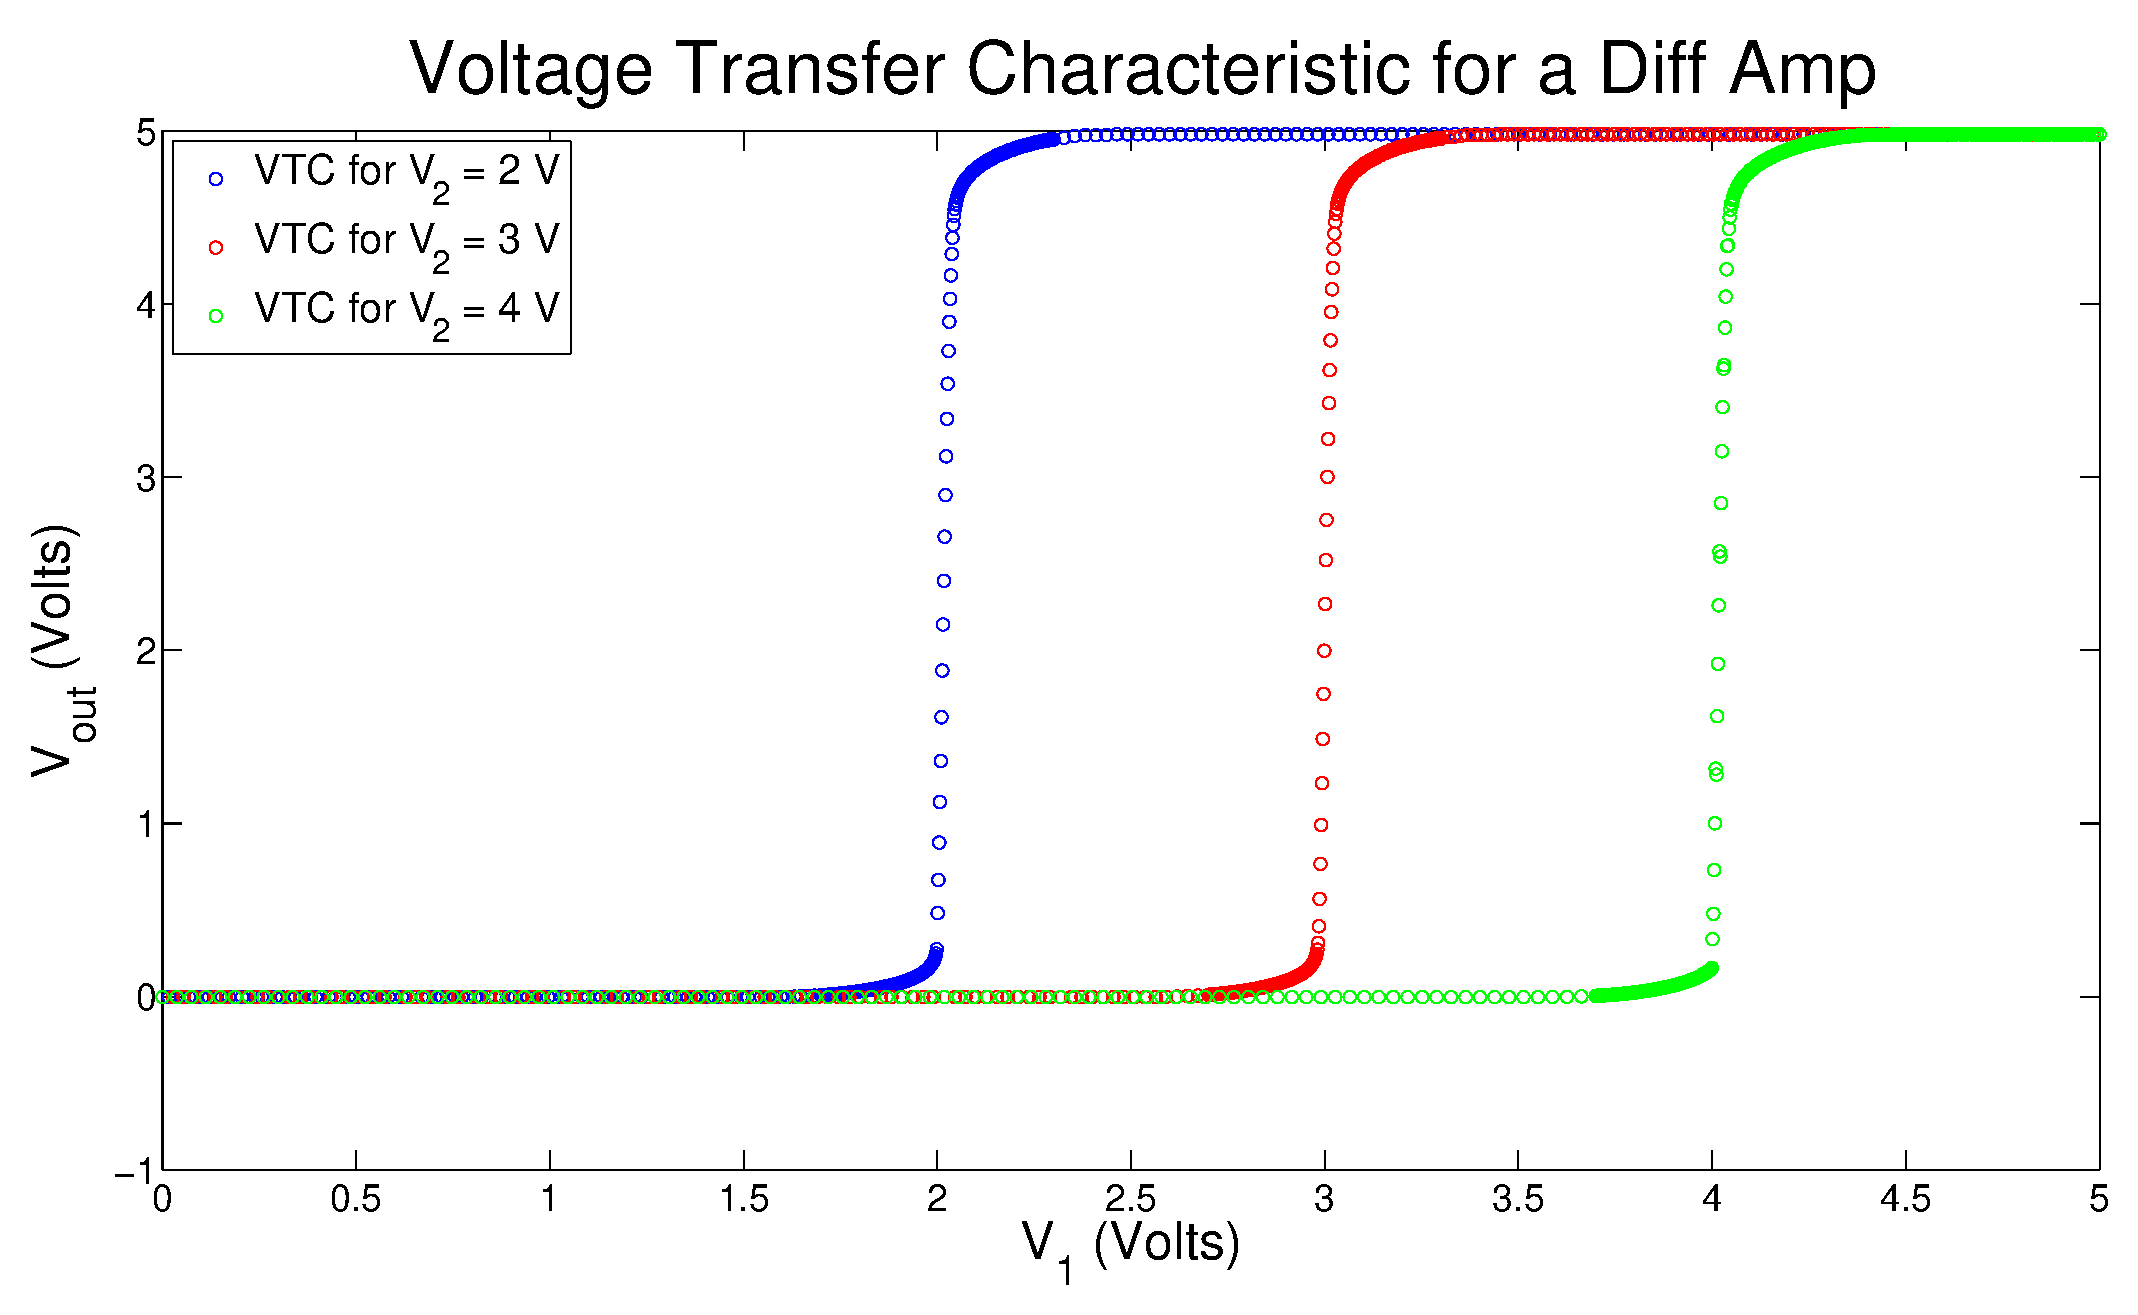
\includegraphics[width=\linewidth]{../Figures/Exp1.eps}
\caption{}
\label{fig:exp1p1}
\end{figure}
The VTC of the improved differential amplifier displays rail-rail operation for all values of \Vone, and a very climb from 0 to \Vdd once $V_1 > V_2$. The transition region between railing low and railing high is approximately 800 mV wide for all three values of \Vtwo. We next compared the VTC of the improved diff amp with the VTC of the diff amp we worked with during Lab 8, which is reproduced in figure \ref{fig:oldvtc} for convenience.
\begin{figure}[H]
\centering
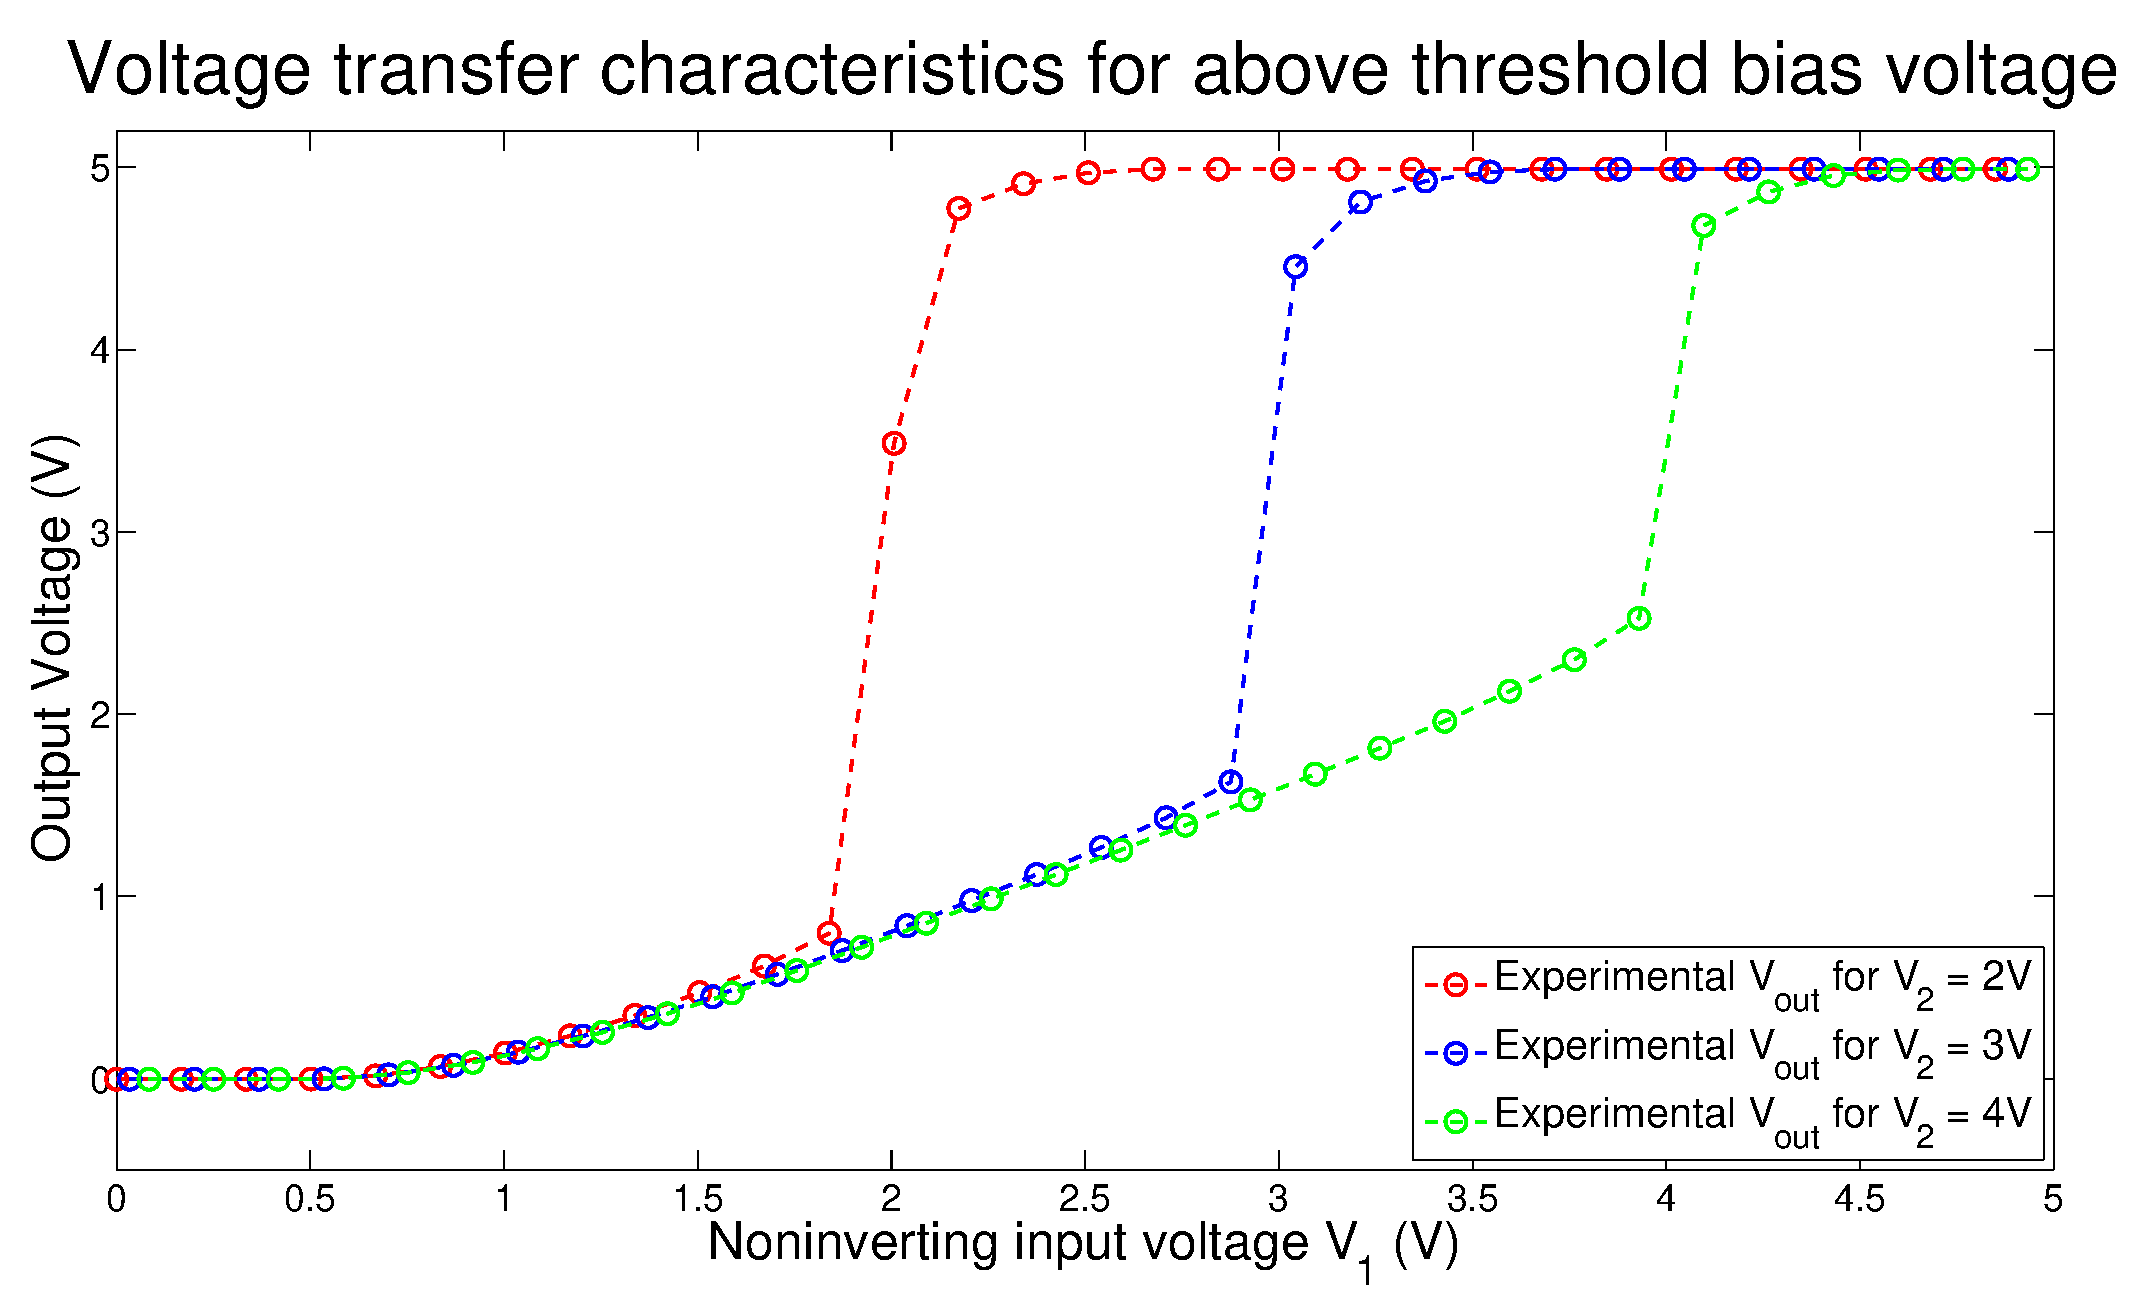
\includegraphics[width=\linewidth]{../Figures/OldVTC.eps}
\caption{}
\label{fig:oldvtc}
\end{figure}

The first obvious different is the poor flooring performance of the old diff amp coompared to the new one. When $V_1 > V_2$, we expect the output to rail low (as we see in figure \ref{fig:exp1p1}), but in the old diff amp \Vout instead followed \Vone linearly, a phenomenon we explained in post-lab 8. The top rail seems to behave the same for both differential amplifiers.

The width of the transition region (from bottom rail to top rail) for the old differential amplifier is far larger, due to the \Vout following \Vone linearly for some values of \Vone. The slope of transition is also less steep, which indicates that the old diff amp is more likely to be stuck between either rail.

The improved diff amp shows better performance characteristics due to the added current mirrors that more effectively isolate the input and output circuitry. The current mirrors prevent the bias transistors from shutting off when \Vout is very high or low, which avoids the \Vout following \Vin linearly for $V_{dm} < 0$, and overall creates a more ideal differential voltage amplifier.